\chapter{Data acquisition for CHIPS} %%%%%%%%%%%%%%%%%%%%%%%%%%%%%%%%%%%%%%%%%%%%%%%%%%%%%%%%%%%%%
\label{chap:daq} %%%%%%%%%%%%%%%%%%%%%%%%%%%%%%%%%%%%%%%%%%%%%%%%%%%%%%%%%%%%%%%%%%%%%%%%%%%%%%%%%

The primary task of any data acquisition system is the processing of low-level signals measuring
real-world physics and their transfer to permanent storage for further analysis. Commonly, this
procedure also includes decision making as to whether the signal is deemed interesting enough to
record, known as a \emph{trigger}. Both of these tasks can make DAQ systems incredibly complex,
especially when they must operate efficiently and resiliently for vast amounts of data in
real-time, whilst also providing detector control and monitoring.

In the context of the \chips project, the DAQ system records all PMT hits, timestamps them using a
common clock, and transfers them out of the detector for processing. A trigger is applied to
select those hits that fall within the interesting \numi beam spill time window before the
selected hits are moved to permanent storage for further analysis. Alongside these processes, the
DAQ system also configures the detector and provides hardware and data quality monitoring.

Although relatively simple when compared to the incredibly complex and time-pressured DAQ systems
of the LHC experiments, the DAQ system developed for the \chips project contains some unique
approaches to solve the goals of the \chips concept. Namely, deployment within a body of water and
a limited resource budget. In this chapter, the DAQ system for \chips as applied to the \chipsfive
prototype detector module is described. The description is presented in two broad categories,
hardware and software, with a short description of the timing system to begin.

The author played a major role in both the development and construction of the DAQ system for
\chipsfive. Specifically, a significant contribution to the development of the networking solution
and high-level hardware implementation was made, alongside building the control and monitoring
software. Furthermore, the author played a role in the development of the novel low-level Madison
$\micro$DAQ and Beaglebone DAQ system.

\section{White Rabbit timing} %%%%%%%%%%%%%%%%%%%%%%%%%%%%%%%%%%%%%%%%%%%%%%%%%%%%%%%%%%%%%%%%%%%%
\label{sec:daq_timing} %%%%%%%%%%%%%%%%%%%%%%%%%%%%%%%%%%%%%%%%%%%%%%%%%%%%%%%%%%%%%%%%%%%%%%%%%%%

To ensure PMT hit times are synchronised throughout \chips detectors, a common clock must be
shared across all timestamping electronics. For this purpose, \chips uses a \emph{White Rabbit}
(WR) network~\cite{lipinski2011}. Initially developed at CERN, the open-source WR project provides
an ethernet-based time distribution network with sub-nanosecond synchronisation accuracy between
nodes. By using two-way exchanges of WR messages, precise adjustment of individual node clock
phases and offsets are possible, across thousands of devices separated by tens of kilometres. All
of this is achieved alongside a standard data transfer network capable of \unit{1}{\text{Gb}}
speeds.

All nodes are synchronised to the clock of a \emph{GrandMaster} node, typically a WR
\emph{switch}, the most common WR hardware component. As input, the GrandMaster switch receives an
IRIG-B (Inter-Range Instrumentation Group timecode B) and a \unit{10}{\text{MHz}} signal from a
GPS disciplined oscillator. These inputs allow for synchronisation of the GrandMaster clock to
International Atomic Time. As \chips detector modules require synchronisation to accelerator
clocks many hundreds of kilometres away to determine the arrival time of beam spills, this GPS
disciplined timing is essential.

WR hardware is commercially available from many vendors. Within \chipsfive, two WR devices are
used for time synchronisation and data transfer, both shown in \FigureRef{fig:wr_electronics}.
Firstly, a compact version of the standard WR switch~\cite{wrswitch2020}, specially developed for
the \chips project at Nikhef~\cite{wrchromium2020}. Secondly, a WR-LEN (Lite Embedded Node) from
Seven Solutions~\cite{wrlen2020}. 

\begin{figure} % WHITE-RABBIT COMPONENTS DIAGRAM %
    \centering
    \subcaptionbox{White Rabbit Switch}{%
        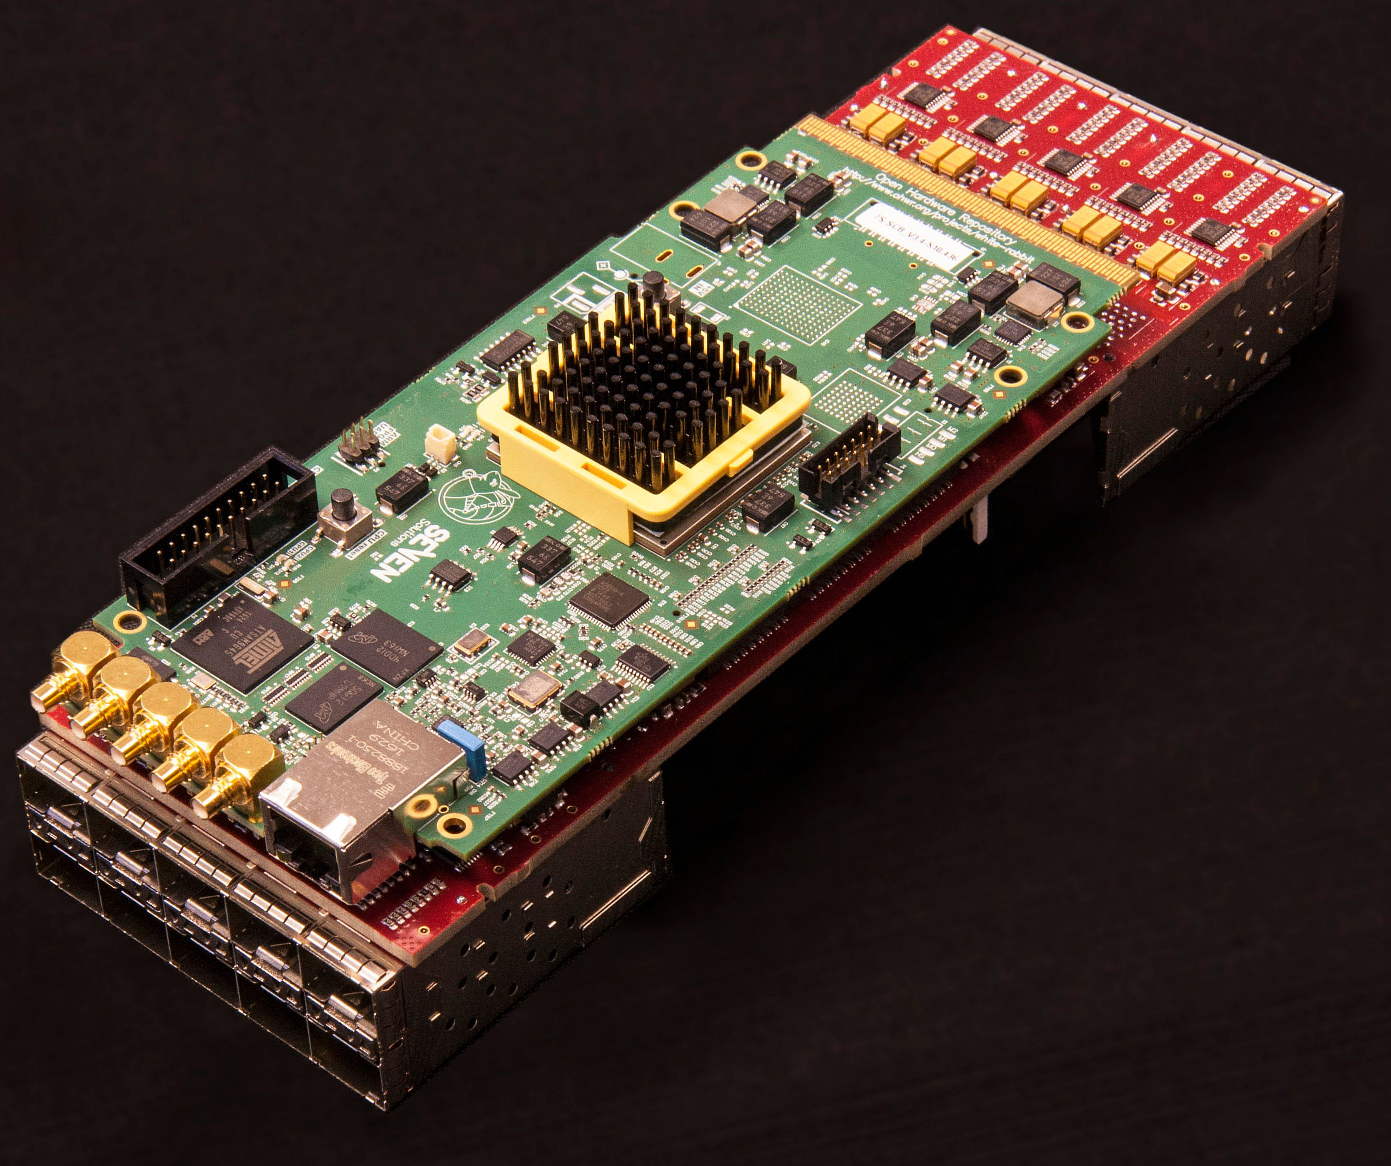
\includegraphics[height=6cm]{diagrams/5-daq/wr_switch.pdf}%
    }
    \quad
    \subcaptionbox{White Rabbit LEN}{%
        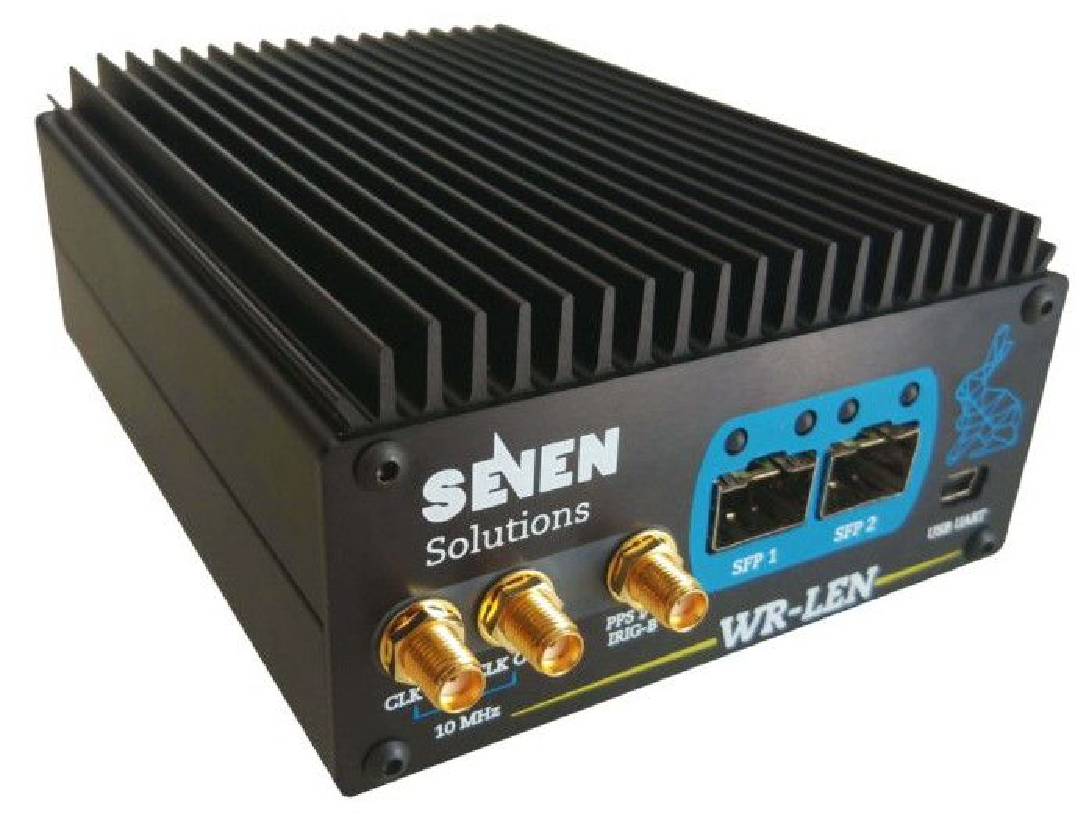
\includegraphics[height=6cm]{diagrams/5-daq/wr_len.pdf}%
    }
    \caption[Pictures of the White Rabbit timing hardware used within \chipsfive]
    {Pictures of the White Rabbit timing hardware used within \chipsfive. The compact WR switch
        specially designed for \chips is shown in (a), while the White Rabbit Lite Embedded Node
        (WR-LEN) from Seven Solutions is shown in (b).}
    \label{fig:wr_electronics}
\end{figure}

All WR components within \chipsfive are connected using \unit{1}{\text{Gb}} bi-directional optical
fibre connections, using the \unit{1310}{\text{nm}} and \unit{1550}{\text{nm}} wavelengths via
Small Form-Factor Pluggable Transceivers (SFPs). \FigureRef{fig:sync} shows the WR synchronised
pulse per second rising edges for two \chipsfive WR switches separated by \unit{500}{\text{m}} of
optical fibre. With the vertical ticks representing single nanoseconds, sub-nanosecond time
synchronisation accuracy between the switches is observed.

\begin{figure} % WHITE-RABBIT SYNC DIAGRAM %
    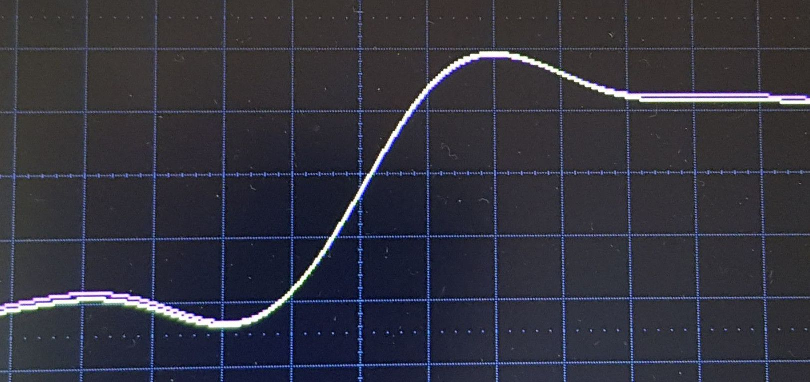
\includegraphics[width=0.7\textwidth]{diagrams/5-daq/sync.pdf}
    \caption[Picture of White Rabbit timing synchronisation seen within \chipsfive]
    {Oscilloscope display measuring the pulse per second output signal from two WR switches shown
        in pink and yellow at either end of a \unit{500}{\text{m}} long optical fibre. The
        vertical ticks are in nanoseconds showing the sub-nanosecond synchronisation possible with
        the WR timing network.}
    \label{fig:sync}
\end{figure}

\section{Hardware} %%%%%%%%%%%%%%%%%%%%%%%%%%%%%%%%%%%%%%%%%%%%%%%%%%%%%%%%%%%%%%%%%%%%%%%%%%%%%%%
\label{sec:daq_hard} %%%%%%%%%%%%%%%%%%%%%%%%%%%%%%%%%%%%%%%%%%%%%%%%%%%%%%%%%%%%%%%%%%%%%%%%%%%%%

The hardware of the \chipsfive DAQ system is split into two distinct implementations at its lower
levels (closest to the PMTs), corresponding to the Nikhef and Madison \textsc{Pom} types. \chips
R\&D efforts have principally developed the novel Madison implementation with the view of using
this hardware exclusively. However, as a safe stepping stone, while development and testing are
still ongoing, \chipsfive mainly contains proven Nikhef hardware developed for the KM3NeT
experiment~\cite{adrian2016}.

The complete DAQ and power distribution system for \chipsfive is diagrammatically shown in
\FigureRef{fig:daq}. The following subsections describe each component, starting from the lowest
level and working upwards. The Nikhef and Madison descriptions are separated for clarity in
addition to the high-level combined hardware systems, part of which is not physically located
within the detector but in an electronics hut onshore.

\begin{figure} % DAQ DIAGRAM %
    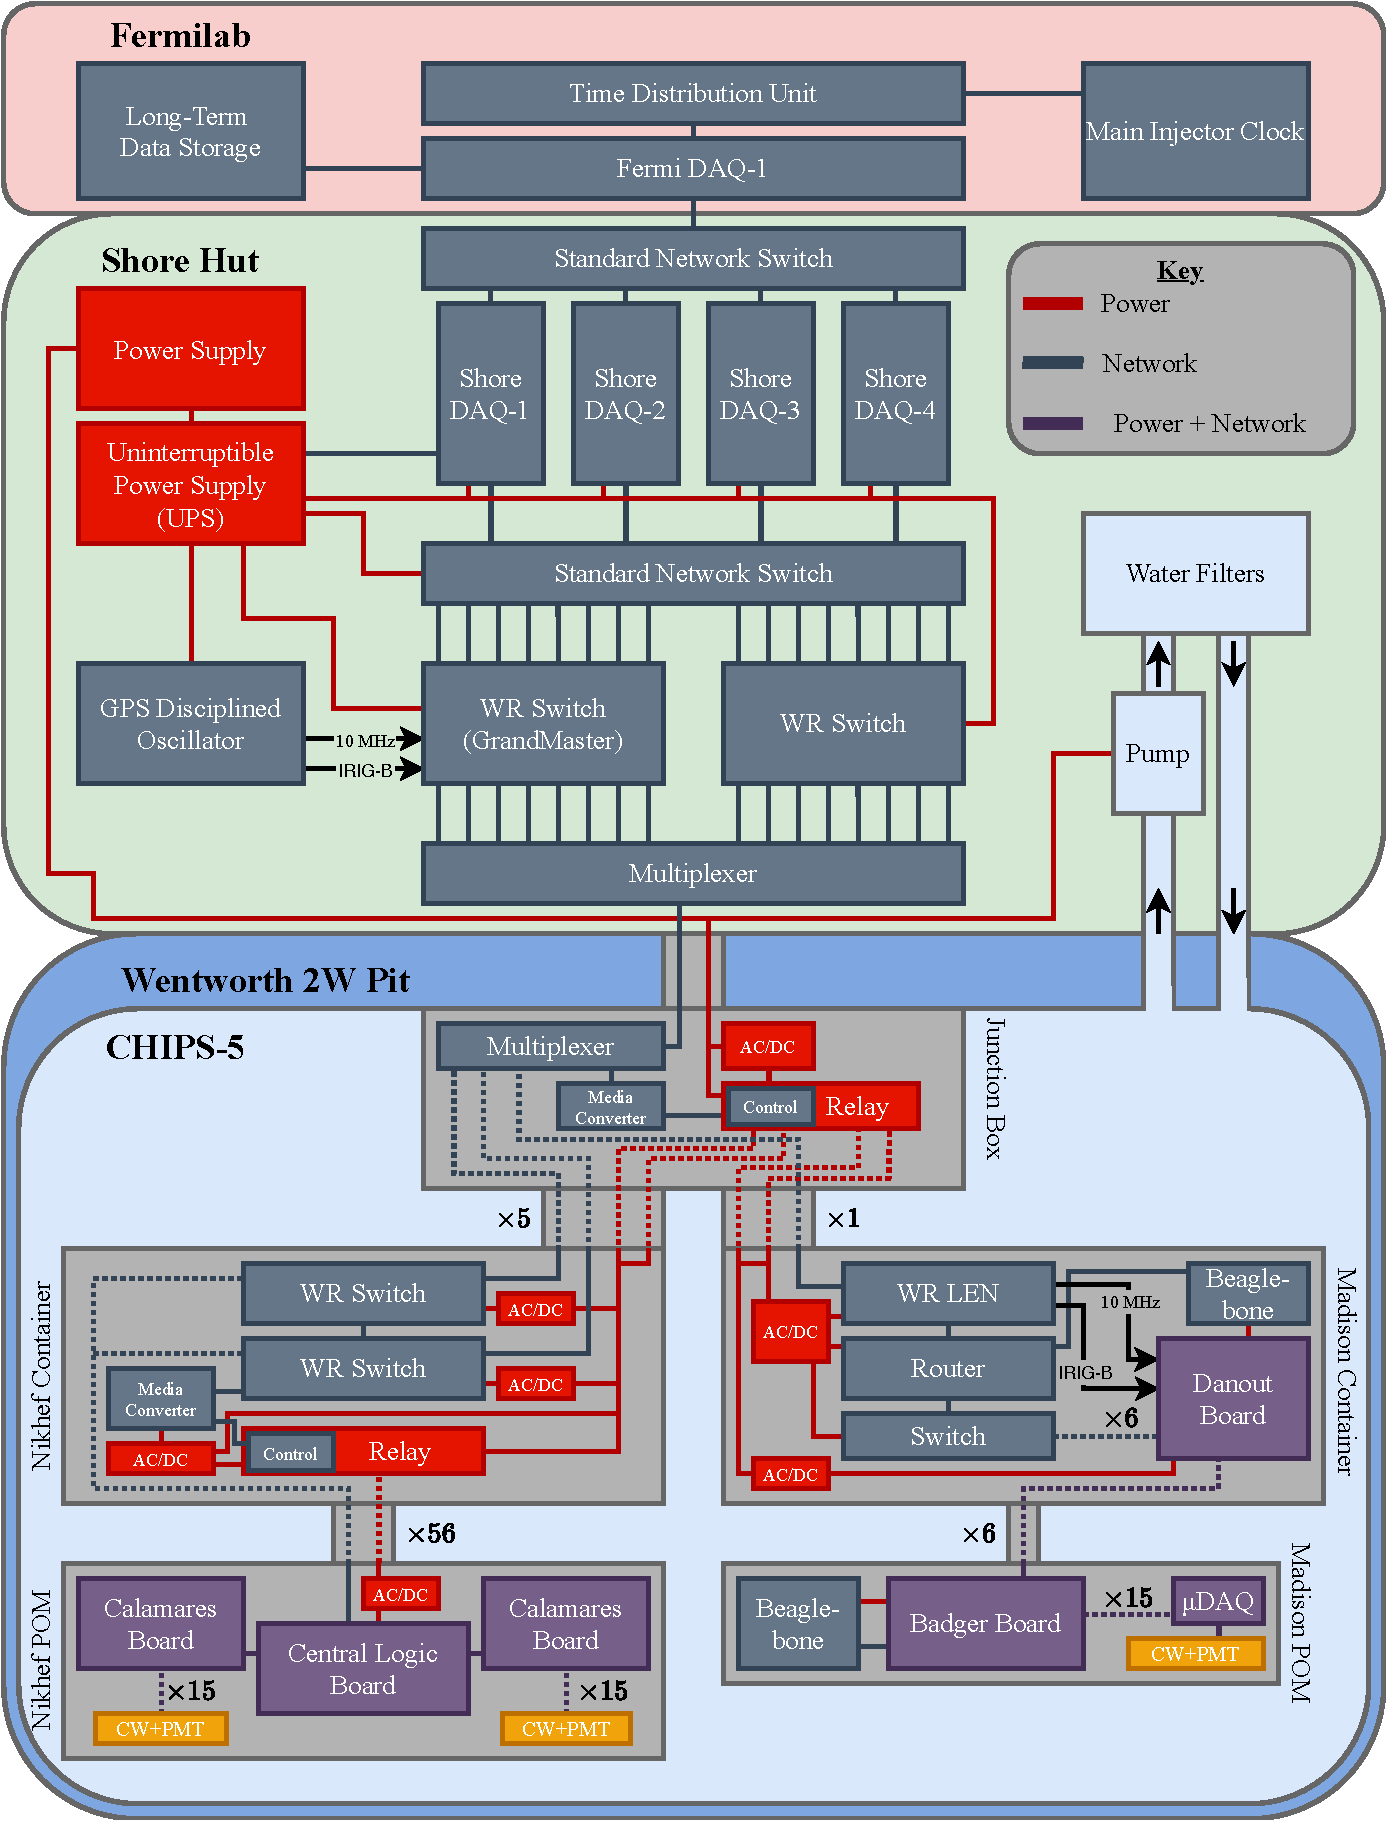
\includegraphics[width=\textwidth]{diagrams/5-daq/daq.pdf}
    \caption[Diagram of the complete \chipsfive data acquisition and power distribution system]
    {Diagram of the complete \chipsfive DAQ and power distribution system.}
    \label{fig:daq}
\end{figure}

As a general overview, the DAQ system within the detector follows a tree-like structure. Starting
from the lowest level (the leaves), individual PMTs are arranged into \textsc{Pom}s. Groups of
\textsc{Pom}s, spatial close within the detector, are then connected to a small number of
group-specific interface containers (either a \emph{Nikhef-container} or
\emph{Madison-container}), holding networking and power supply devices for each group. All
interface containers are attached to a central aggregation box (\emph{junction-box}) which feeds
connections into a single umbilical (the tree trunk) to shore.

Common to both low-level hardware implementations is the use of the Time over Threshold (ToT)
method for PMT signal digitisation. Each analogue PMT pulse is fed to a ToT discriminator coupled
with a Time to Digital Converter (TDC) to generate each digitised recorded hit, as shown in
\FigureRef{fig:tot}. Compared to the more common Analogue to Digital Converter (ADC) readout, ToT
values are less accurate and do not scale linearly with deposited charge. However, as the maximum
expected deposited charge within \chips detectors is relatively low (only a few p.e), the impact
of the non-linearity is small, and the ToT implementation is used. Furthermore, ToT electronics
are simpler and notably cheaper.

\begin{figure} % TOT DIAGRAM DIAGRAM %
    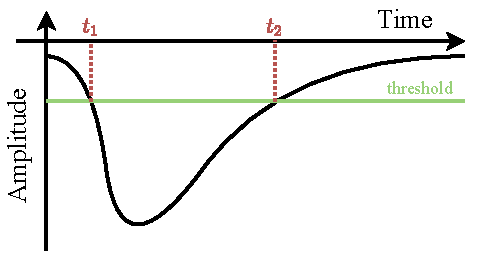
\includegraphics[width=0.6\textwidth]{diagrams/5-daq/tot.pdf}
    \caption[Illustrative diagram showing how Time over Threshold is measured]
    {Illustrative diagram showing how a ToT value is measured. As soon as the rising edge of a PMT
        charge pulse rises above a given threshold (goes below in the negative charge case) a time
        is recorded $t_{1}$, when the falling edge later falls below the threshold a second time
        $t_{2}$ is recorded. The difference in time between $t_{1}$ and $t_{2}$ is output by the
        electronics as a digitised ToT value.}
    \label{fig:tot}
\end{figure}

\subsection{Nikhef hardware} %%%%%%%%%%%%%%%%%%%%%%%%%%%%%%%%%%%%%%%%%%%%%%%%%%%%%%%%%%%%%%%%%%%%%
\label{sec:daq_hard_Nikhed} %%%%%%%%%%%%%%%%%%%%%%%%%%%%%%%%%%%%%%%%%%%%%%%%%%%%%%%%%%%%%%%%%%%%%%

All Nikhef HZC PMTs are attached directly to a simple readout board containing a high-voltage
generating Cockcroft-Walton circuit~\cite{cockcroft1932}. Up to 30 such PMTs are connected to two
fanout \emph{Calamares} boards within the electronics box of each Nikhef \textsc{Pom} via standard
cables with RJ45 connectors, as shown in \FigureRef{fig:nikhef_plane}. Both Calamares boards are
directly attached to a \emph{Central Logic Board} (CLB)~\cite{biagi2015, eijk2015}. The CLB
contains the ToT discriminators and TDCs used to digitise the recorded signals, as well as an FPGA
(Field-Programmable Gate Array) programmed to provide additional logic and WR clock
synchronisation for timestamping. Each Nikhef \textsc{Pom} electronics box also contains an AC to
DC power converter (AC/DC) whose output is fed into the CLB for distribution.

\begin{figure} % NIKHEF PLANE DIAGRAM %
    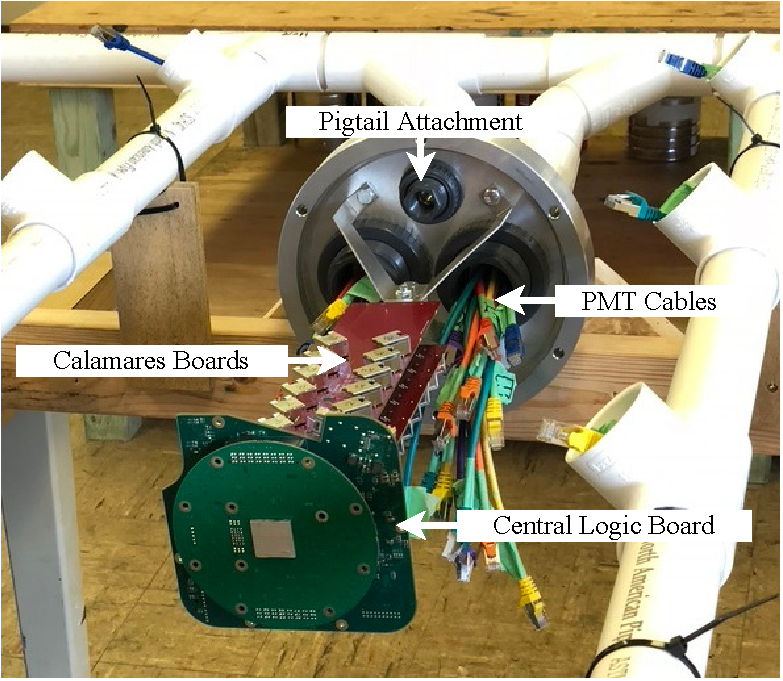
\includegraphics[width=0.8\textwidth]{diagrams/5-daq/nikhef_plane.pdf}
    \caption[Labelled picture of the Nikhef \textsc{Pom} electronics box]
    {Labelled picture of the Nikhef \textsc{Pom} electronics box without its aluminium casing.
        Both ends of the PMT cables can be seen, either at the PMT mounting points or entering the
        electronics box and not yet plugged into Calamares boards.}
    \label{fig:nikhef_plane}
\end{figure}

Every Nikhef \textsc{Pom} is connected via a single optical fibre and a single power connection to
an interface Nikhef-container, the contents of which are labelled in the bottom half of
\FigureRef{fig:full_setup}. An aluminium structure holds two WR switches within each container
specially designed to remove heat from the switch components and transfer it to the colder outer
shell. Both switches are powered by independent AC to DC converters and connected via a single
optical fibre each to the higher level DAQ systems. An additional connection is made between each
switch to ensure that if one higher-level connection fails, the other can still be used for
networking.

Each Nikhef-container also holds a relay board to control the power supply to individual
\textsc{Pom}s. The relay board control electronics are powered via an AC to DC converter and
connected to one of the switches via a media converter for networking. The media converter is
required to convert the optical fibre WR switch connection to a standard RJ45 copper cable
connection. A total of five Nikhef-containers are present within \chipsfive.

\begin{figure} % FULL SETUP DIAGRAM %
    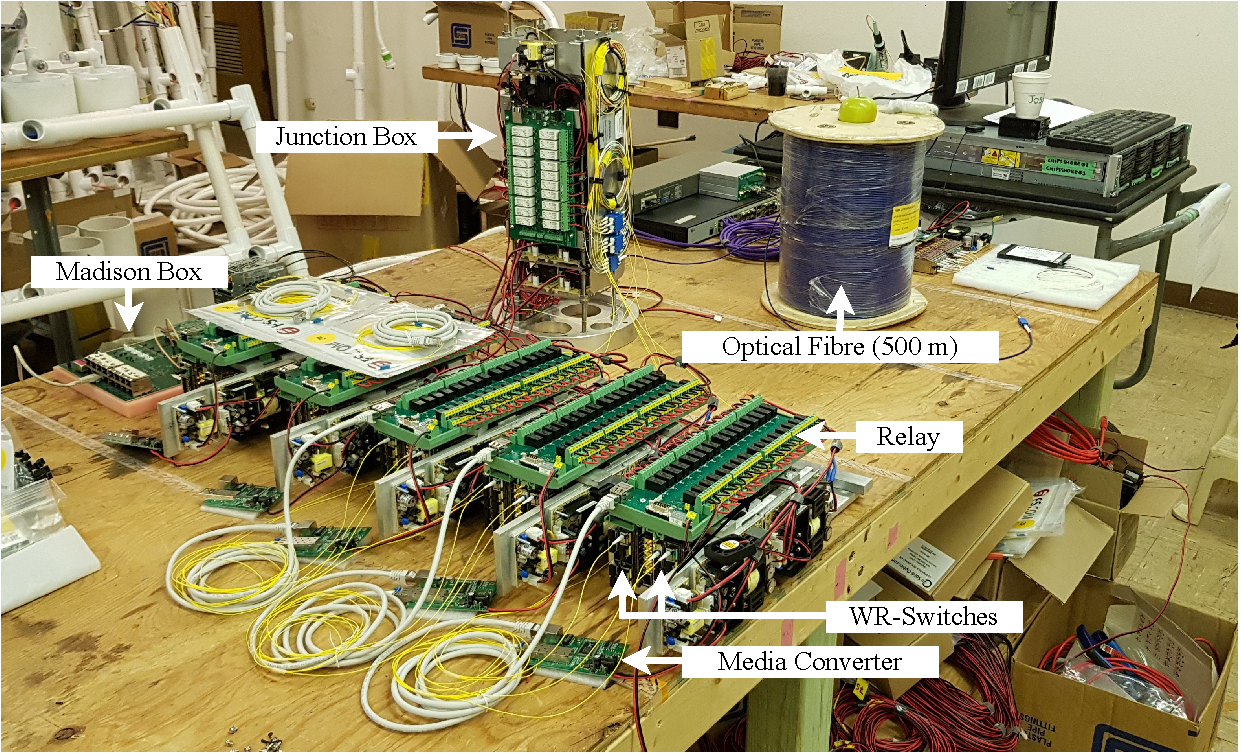
\includegraphics[width=\textwidth]{diagrams/5-daq/full_setup.pdf}
    \caption[Labelled picture of the high-level components of the \chipsfive DAQ system]
    {Labelled picture of the high-level non \textsc{Pom} components of the \chipsfive DAQ system
        arranged on a table at the PolyMet mining administration building.}
    \label{fig:full_setup}
\end{figure}

\subsection{Madison hardware} %%%%%%%%%%%%%%%%%%%%%%%%%%%%%%%%%%%%%%%%%%%%%%%%%%%%%%%%%%%%%%%%%%%%
\label{sec:daq_hard_madison} %%%%%%%%%%%%%%%%%%%%%%%%%%%%%%%%%%%%%%%%%%%%%%%%%%%%%%%%%%%%%%%%%%%%%

Every Madison Hamamatsu PMT is directly attached to a high-voltage generating Cockcroft-Walton
board followed by a signal processing $\micro$DAQ, as shown in
\FigureRef{fig:madison_pmt_assembly}. The $\micro$DAQ is a small microcontroller developed for
both IceCube and \chips at WIPAC in Madison. Capable of timestamping and digitising signals
directly at the PMT level, the $\micro$DAQ also sets the PMT operating voltage by controlling the
driving frequency of the Cockcroft-Walton board~\cite{eijk2018}.

Up to 16 $\micro$DAQs receive power, networking, and WR synchronised IRIG-B and
\unit{10}{\text{MHz}} timing signals from a \emph{badger-board}, as shown in
\FigureRef{fig:madison_plane}. Standard cables with RJ45 connectors are used for these
connections. The badger-board is located within the electronics box of each Madison \textsc{Pom}
and acts as a simple fanout and power control board. For logic, each badger-board has an attached
mezzanine Beaglebone~\cite{beagle2020}. This single-board Linux machine (very similar to a
Raspberry Pi) controls the power supply to, and receives hits from, the attached $\micro$DAQs.

\begin{figure} % MADISON PLANE DIAGRAM %
    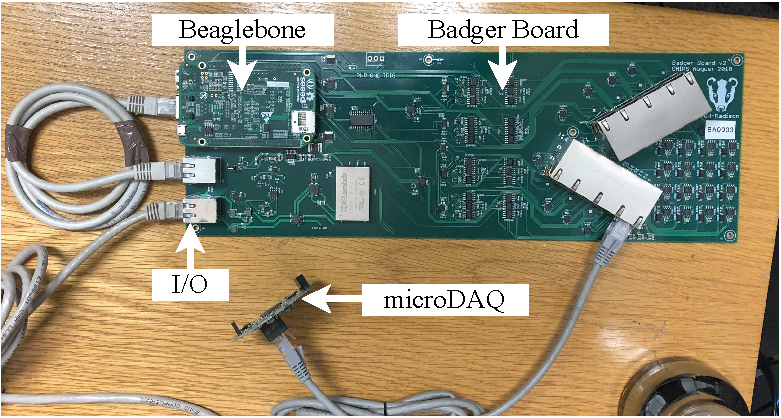
\includegraphics[width=0.8\textwidth]{diagrams/5-daq/madison_plane.pdf}
    \caption[Labelled picture of the components of the Madison \textsc{Pom} electronics box]
    {Labelled picture of the components of the Madison \textsc{Pom} electronics box.}
    \label{fig:madison_plane}
\end{figure}

Similarly, up to 16 Madison \textsc{Pom} badger-boards receive power, networking, and WR
synchronised IRIG-B and \unit{10}{\text{MHz}} timing signals from a \emph{danout-board} located
within a single interface Madison-container. Again, standard cables with RJ45 connectors are used
for these connections. The full contents of the Madison-container are shown in
\FigureRef{fig:madison_box}. Similar to the badger-board, the danout-board acts as a simple fanout
and power control board with an attached mezzanine Beaglebone. However, in this case, the attached
Beaglebone acts only to control the power provided by the danout-board.

PMT hits and other data are instead routed through the danout-board into a networking stack.
Consisting of a WR-LEN, a router (required due to the limited WR-LEN routing table size), and a
switch (non-WR), the stack provides networking to the higher-level DAQ via a single optical fibre.
The WR clock synchronised IRIG-B and \unit{10}{\text{MHz}} timing signals are output by the WR-LEN
to the danout-board for forwarding to the lower-level components. Additionally, two AC to DC
converters provide power for both the devices within the container and all lower-level components
via the danout-board.

\begin{figure} % MADISON BOX DIAGRAM %
    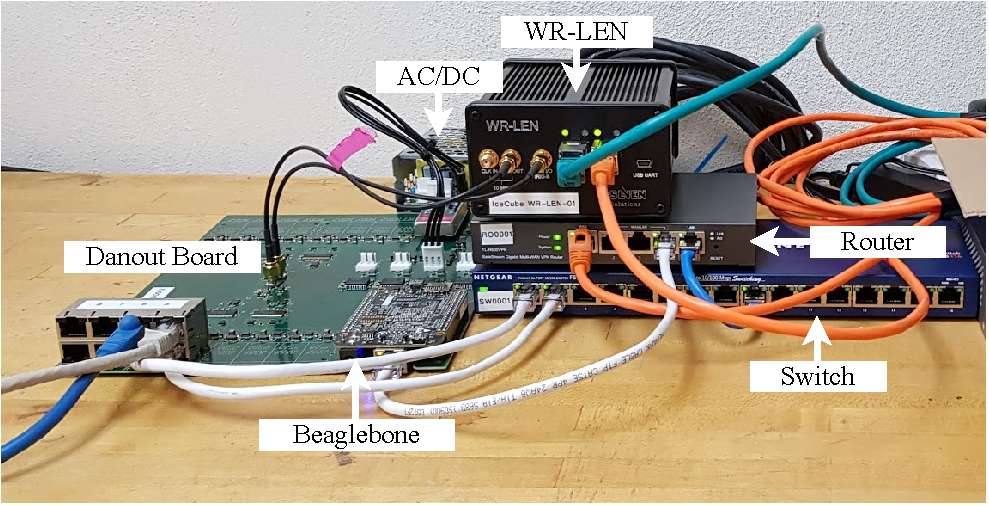
\includegraphics[width=\textwidth]{diagrams/5-daq/madison_box.pdf}
    \caption[Labelled picture of the Madison-container components]
    {Labelled picture of the Madison-container components. The blue and grey cables exiting the
        left hand side of the image go to individual Madison \textsc{Pom}s connecting to the I/O
        port shown in \FigureRef{fig:madison_plane}. An optical fibre connection into the left SFP
        port of the WR-LEN is used in reality rather than the copper connection shown here.}
    \label{fig:madison_box}
\end{figure}

Compared to the Nikhef hardware the \chips developed Madison implementation has a few key
advantages, primarily driven by the core \chips concept of reducing cost:
\begin{itemize}
    \item Commercially available and cheap ($\sim\textsterling50$ each) Beaglebones are leveraged
    for \textsc{Pom} level processing and logic instead of expensive, FPGA based CLBs. Not only
    are they cheap but Beaglebones provide a fully configurable general-purpose Linux machine that
    can easily be enhanced with new features once deployed. This is in comparison to CLBs which
    can be only be reconfigured via remote reprogramming of the FPGA.

    \item PMT hit processing and logic is pushed right to the lowest-level PMTs themselves via the
    use of $\micro$DAQs. Although not currently fully realised this can have significant
    implications for the DAQ system as a whole. For example, future updates will allow for beam
    spill hit triggering to be performed on the $\micro$DAQ, drastically reducing the capacity
    requirements of the rest of the DAQ system, further reducing costs.

    \item The number of expensive WR switches is reduced, with much cheaper WR-LENs taking their
    place. Although this change removes WR clock time synchronisation from the \textsc{Pom} level,
    tests have shown that achievable cable length time corrections still allow for sub-nanosecond
    synchronisation accuracy to be reached.
\end{itemize}

\subsection{Combined systems} %%%%%%%%%%%%%%%%%%%%%%%%%%%%%%%%%%%%%%%%%%%%%%%%%%%%%%%%%%%%%%%%%%%%
\label{sec:daq_hard_combined} %%%%%%%%%%%%%%%%%%%%%%%%%%%%%%%%%%%%%%%%%%%%%%%%%%%%%%%%%%%%%%%%%%%%

Each interface container is connected to a single junction-box, labelled in
\FigureRef{fig:full_setup}. This central container acts as the interface between the detector
electronics and the umbilical, carrying data and power between the shore and the detector. 

Due to the unique \chips constraint of complete submersion within water, all connections to the
junction-box (as well as those between \textsc{Pom}s and the interface containers) are made within
watertight, flexible PVC tubing called \emph{manifolds}. These tubes span all corners of the
\chipsfive detector, as shown in \FigureRef{fig:manifold}, usually attached to the endcap frames.
Additionally, as is done for the individual \textsc{Pom}s, water-blocks are placed between all
interface containers and the junction-box to compartmentalise the higher-level DAQ components and
prevent a single leak from taking down the whole system.

\begin{figure} % MANIFOLD DIAGRAM %
    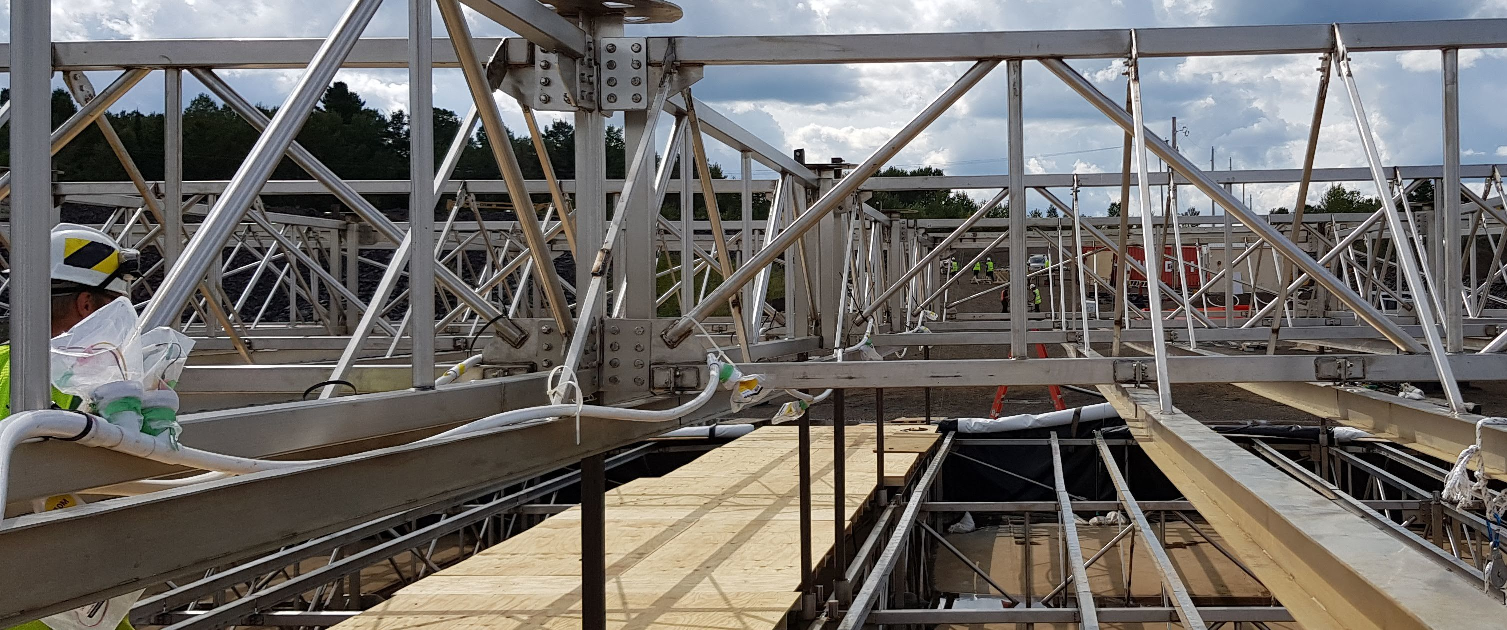
\includegraphics[width=\textwidth]{diagrams/5-daq/manifold.pdf}
    \caption[Picture of a manifold connection within the \chipsfive detector]
    {Picture of a Nikhef \textsc{Pom} to Nikhef-container manifold (in white) attached to the
        top-cap of the \chipsfive detector. In the left of the image, two unattached Nikhef
        \textsc{Pom} pigtail connections are seen, both covered in green tape and a plastic bag.
        The manifolds can also be seen in the graphical rendering of the top-cap shown in
        \FigureRef{fig:top_cap}.}
    \label{fig:manifold}
\end{figure}

For networking the junction-box contains a Coarse Wavelength Division Multiplexing (CWDM)
multiplexer/demultiplexer (MUX/DEMUX). This device supports 32 wavelengths for a total of 16
bi-directional \unit{1}{\text{Gb}} connections over the single \unit{500}{\text{m}} long umbilical
optical fibre. Each WR-LEN or WR switch within the detector uses one of these channels exclusively
with the corresponding wavelength SFP.

The two umbilical power connections are distributed via two thick copper plates to all the relay
channels within the junction-box. Two relay boards are used to provide a sufficient number of
output channels, with their control electronics powered by separate AC to DC converters and each
connected to one of the MUX/DEMUX networking channels via a media converter (optical fibre to
RJ45). Each relay channel also has a built-in \emph{trip gate} to immediately power-off the
channel if a current surge is detected. This protection is particularly crucial for \chipsfive as
water leaks are possible.

The contents of the DAQ electronics \emph{Shore Hut} are shown in \FigureRef{fig:hut_daq}. The
single umbilical optical fibre connection passes through a MUX/DEMUX before each of the
wavelength-specific channels are passed into one of two WR switches. Multiple Virtual Local Area
Networks (VLANs) are configured on each switch such that for each wavelength channel only a single
paired port on the other physical side of the switch carries that channels data to and from the
standard networking switch (these connections are not present within \FigureRef{fig:hut_daq}). Of
the two WR switches, one is configured to be the GrandMaster with connections to a GPS disciplined
oscillator. A single connection is also made between the WR switches for clock synchronisation.

\begin{figure} % WHITE-RABBIT GM SETUP DIAGRAM %
    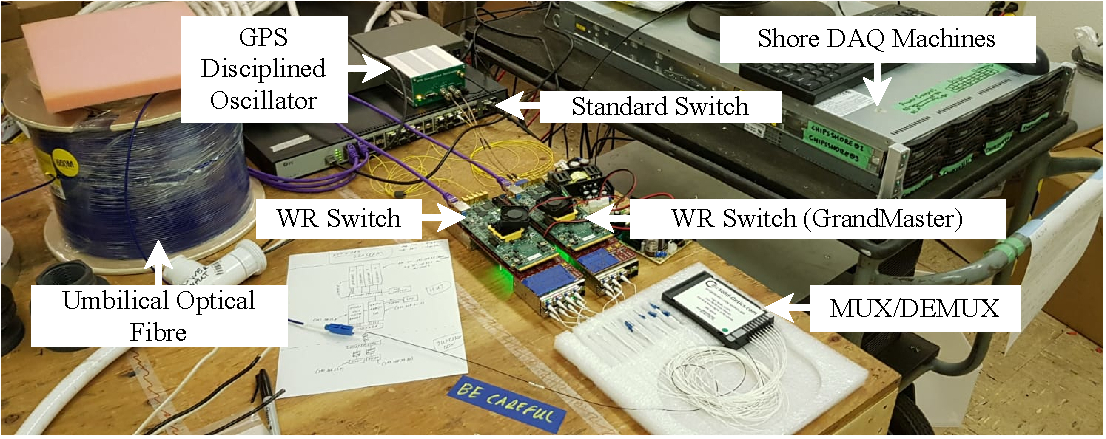
\includegraphics[width=\textwidth]{diagrams/5-daq/hut_daq.pdf}
    \caption[Labelled picture of the high-level onshore components of the \chipsfive DAQ system]
    {Labelled picture of the high-level onshore components of the \chipsfive DAQ system arranged
        on a table at the PolyMet mining administration building.}
    \label{fig:hut_daq}
\end{figure}

The standard network switch provides \unit{10}{\text{Gb}} connections to each of the Shore DAQ
computing machines whose specific roles are detailed in \SectionRef{sec:daq_soft}. Each machine is
also connected to a second switch providing connections to the external internet and DAQ
components located at Fermilab. At Fermilab, a DAQ machine (Fermi DAQ-1) performs two main roles.
Firstly, it forwards \numi beam spill timing information from a Time Distribution Unit attached to
the Main Injector clock to \chipsfive. Secondly, it receives recorded detector data and places it
into long-term storage.

An uninterruptible power supply provides power to all devices within the Shore Hut, supplying
power for up to \unit{15}{\text{minutes}} after a power cut, sadly quite a common occurrence. This
protection gives all Shore Hut devices plenty of time to appropriately close any open data files
and power down safely. The two detector umbilical power connections do not use the uninterruptible
supply and instead draw power directly from the master supply.

\section{Software and the flow of data} %%%%%%%%%%%%%%%%%%%%%%%%%%%%%%%%%%%%%%%%%%%%%%%%%%%%%%%%%%
\label{sec:daq_soft} %%%%%%%%%%%%%%%%%%%%%%%%%%%%%%%%%%%%%%%%%%%%%%%%%%%%%%%%%%%%%%%%%%%%%%%%%%%%%

The software of the \chipsfive DAQ system provides three main functionalities: control of the
detector instrumentation, the handling of recorded PMT hits, and the monitoring of hardware and
data quality. Each of these functions are discussed within a specific subsection below alongside
the corresponding software processes (applications) that perform them. Only the high-level
software components (physically processed onshore) are detailed, with the low-level CLB,
Beaglebone, and $\micro$DAQ software implementations omitted for brevity. An in-depth discussion
of the CLB software can be found in \ReferenceRef{aiello2019}, while the Beaglebone and
$\micro$DAQ software implementation can be found at \ReferenceRef{microdaq2020}.

\begin{figure} % SOFTWARE DIAGRAM %
    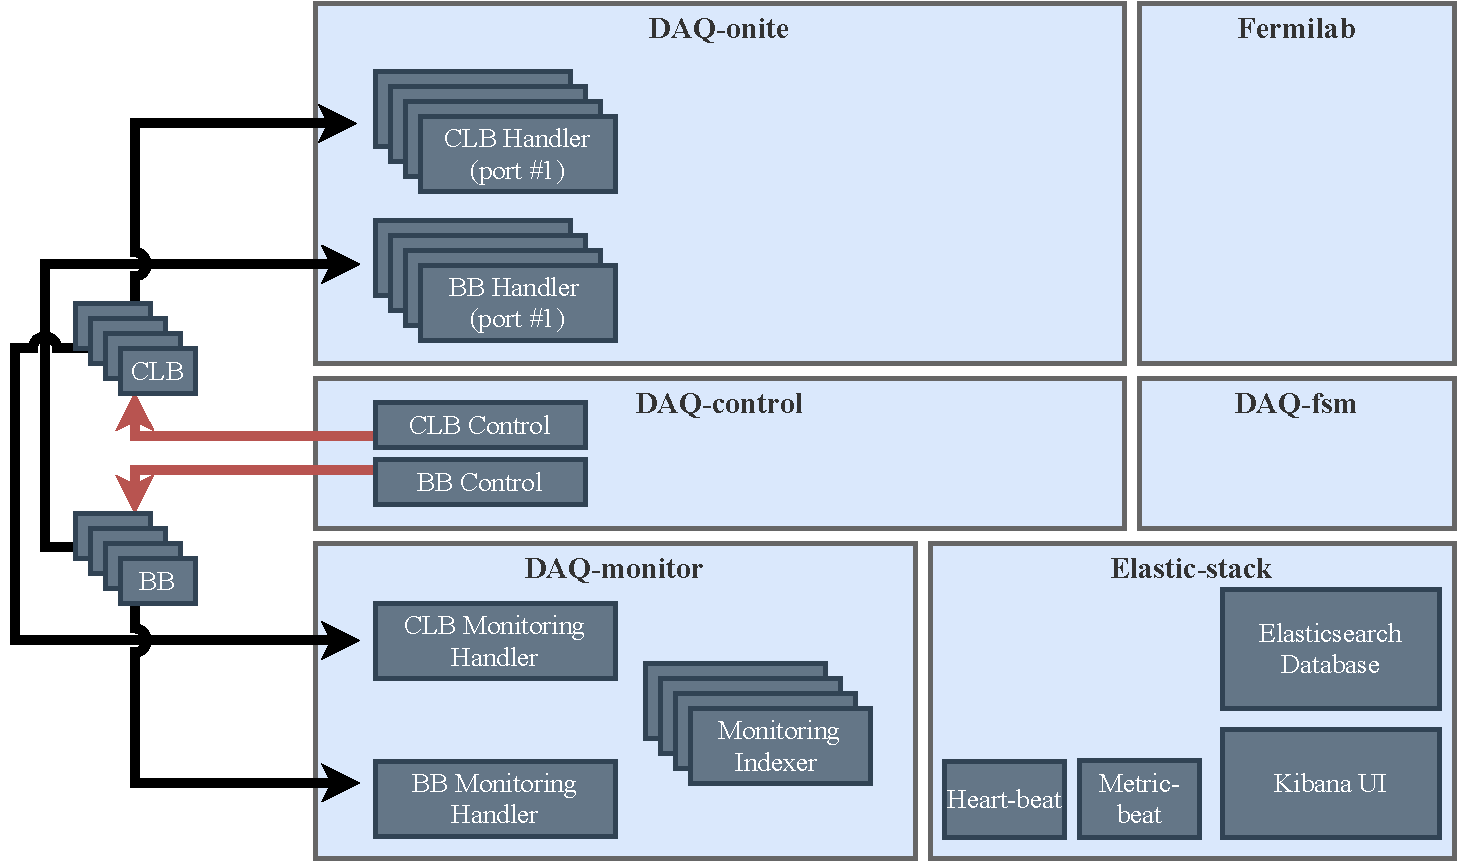
\includegraphics[width=\textwidth]{diagrams/5-daq/daq_software.pdf}
    \caption[Diagram of the \chipsfive software system in terms of the flow of data between
    components] {Diagram of the \chipsfive software system in terms of the flow of data between
    components. Beaglebone is abbreviated to BB.}
    \label{fig:daq_software}
\end{figure}

The DAQ software itself is mainly written in C++ and can be found at \ReferenceRef{chipsdaq2020}.
The system is comprised of multiple processes containing multiple components each (usually
processed on separate threads), as is shown within \FigureRef{fig:daq_software}, expressed in
terms of the flow of data between components. All DAQ processes make extensive use of
multithreading and asynchronous communication, principally implemented using the low-level Boost
Asio (asynchronous input/output) library~\cite{boost2020}. 

All high-level processing takes place on one of three machines: Shore DAQ-1 for hit handling,
Shore DAQ-2 for control and monitoring, and Fermi DAQ-1 for \numi spill forwarding and storage. As
the processing of PMT hits is the principal software task, hit handling takes place exclusively on
Shore DAQ-1 to ensure maximum available processing power. Both Shore DAQ machines have a
corresponding backup machine (Shore DAQ-3 and Shore DAQ-4) to take over their functions
immediately in case of a fault.

\subsection{Control} %%%%%%%%%%%%%%%%%%%%%%%%%%%%%%%%%%%%%%%%%%%%%%%%%%%%%%%%%%%%%%%%%%%%%%%%%%%%%
\label{sec:daq_soft_control} %%%%%%%%%%%%%%%%%%%%%%%%%%%%%%%%%%%%%%%%%%%%%%%%%%%%%%%%%%%%%%%%%%%%%

All DAQ processes and low-level DAQ devices (CLBs and Beaglebones) conform to a global Finite
State Machine (FSM) schema. The schema defines a finite set of states, shown in
\FigureRef{fig:fsm}, for which a DAQ process can only be in one at any given time. Specifically
allowed transitions, triggered by a command signal, allow each process to move between states.
During transition, the process performs the specific actions required to achieve the desired
state. Every DAQ process makes its current internal state publicly known via constant publishing
over a standard inter-process communication socket (Unix domain socket).

\begin{figure} % FSM DIAGRAM %
    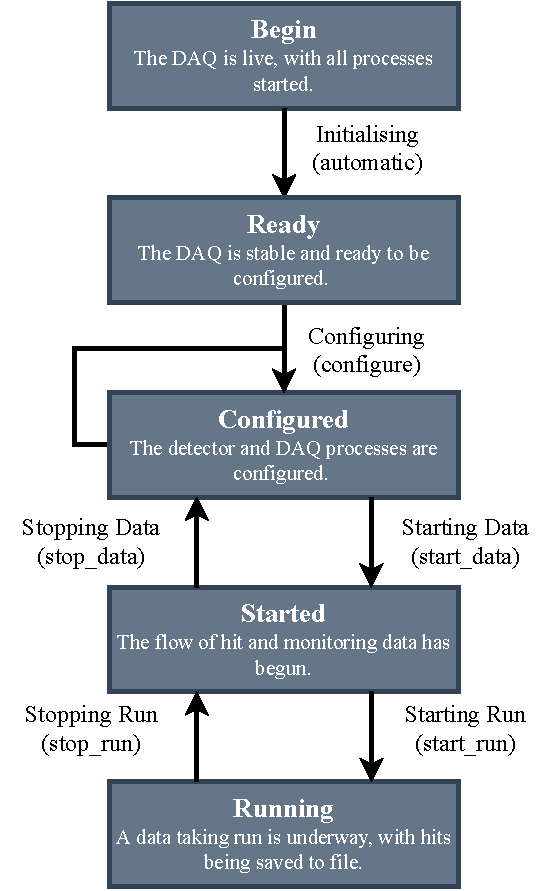
\includegraphics[width=0.4\textwidth]{diagrams/5-daq/fsm.pdf}
    \caption[Diagram of the allowed states and transitions of the \chipsfive Finite State Machine]
    {Diagram of the allowed states and transitions of the \chipsfive FSM. The command signal names
    for each transition are shown in brackets.}
    \label{fig:fsm}
\end{figure}

A singleton \emph{FSM} process both issues the transition signals to and monitors the state of all
DAQ processes. The FSM process defines the global state of the DAQ system, only transitioning to a
new state once all children DAQ processes have reached the desired state. Currently, no control
scheduling system is implemented to automatically configure the detector and conduct a given set
of runs. Therefore, a simple command-line interface is used to issue state transition commands to
the FSM process manually. Viewing the DAQ system as a whole, the actions performed at each state
transition are as follows:
\begin{itemize}
    \item \textbf{Initialising} occurs automatically when the DAQ system is started. During this
    transition all processes conduct the basic actions required for them to be able to function,
    such as opening inter-process communication channels, validating CLB and Beaglebone
    connections, and starting worker threads.
    \item \textbf{Configuring} occurs when the \emph{configure} command is issued. During this
    transition the desired detector configuration is read from a human-readable file and all DAQ
    devices configured accordingly. This procedure primarily consists of setting the desired
    high-voltage level and ToT thresholds for each PMT via communication with all CLBs and
    Beaglebones.
    \item \textbf{Starting Data} occurs when the \emph{start\_data} command is issued. During this
    transition commands are sent to all CLBs and Beaglebones to start the flow of PMT hit and
    monitoring data.
    \item \textbf{Stopping Data} occurs when the \emph{stop\_data} command is issued. During this
    transition commands are sent to all CLBs and Beaglebones to stop the flow of PMT hit and
    monitoring data.
    \item \textbf{Starting Run} occurs when the \emph{start\_run} command is issued. During this
    transition the handling of PMT hit data is started, with the resulting data saved to file.
    This procedure includes the selection of hits according to the \numi beam spill trigger, as
    detailed in \SectionRef{sec:daq_soft_hits}.
    \item \textbf{Stopping Run} occurs when the \emph{stop\_run} command is issued. During this
    transition the handling of PMT hit data is stopped, and the run data file closed.
\end{itemize}

For control of the detector devices, a \emph{DAQ-control} process issues commands to and monitors
the state of all CLBs and Beaglebones. For communication, all messages are exchanged using
standard TCP (Transmission Control Protocol) packets over ethernet. A DHCP server on Shore DAQ-2
assigns predefined static IP addresses to all devices to allow this to happen easily. 

A single DAQ-control controller thread receives commands from the FSM process and instructs
separate CLB and Beaglebone controller threads to issue the appropriate implementation-specific
`slow-control' commands for the given transition. A simple retry mechanism ensures that multiple
attempts are made to achieve the desired state on each device. However, a CLB or Beaglebone is
dropped after a maximum number of attempts have been made in order not to block the global DAQ
transition due to a single faulty device.

\subsection{Hit handling} %%%%%%%%%%%%%%%%%%%%%%%%%%%%%%%%%%%%%%%%%%%%%%%%%%%%%%%%%%%%%%%%%%%%%%%%
\label{sec:daq_soft_hits} %%%%%%%%%%%%%%%%%%%%%%%%%%%%%%%%%%%%%%%%%%%%%%%%%%%%%%%%%%%%%%%%%%%%%%%%

As is done within the KM3NeT experiment, an `all-data-to-shore' approach to PMT hit acquisition is
taken, where all recorded hit data is sent via the WR network to the machines onshore. No
triggering takes place within the detector. This is conducted by collecting all PMT hits within
\unit{10}{\text{ms}} long time windows. At the end of each window, collected hits are packaged
along with a header into UDP (User Datagram Protocol) packets and sent to shore. This process
occurs on both the CLBs and Beaglebones when in either the \emph{Started} or \emph{Running} FSM
state.

Jumbo UDP packets of maximum size \unit{9000}{\text{bytes}} are used instead of typical
\unit{1500}{\text{byte}} packets. This is done to both reduce the proportion of bandwidth taken up
by headers, and reduce the total network traffic (number of packets), leading to a decrease in the
overall proportion of dropped packets. Although UDP does not contain the error-checking and
correction features built into TCP, the proportion of lost packets is negligible and the increased
bandwidth desirable.

PMT hit packets are handled by the \emph{DAQ-onite} process, named after the Taconite ore that
used to be extracted from the Wentworth 2W pit. The primary function of DAQ-onite is to store
incoming PMT hits whose timestamp matches a \numi beam spill trigger window and discard those that
do not. This is complicated by the fact that the exact \numi spill time is not known in advance. 

Whenever the Main Injector at Fermilab releases a spill of protons for the \numi beam, the
accurate timestamp of this event is only published as it happens. Therefore, by the time the
Fermilab based \emph{Spill Server} and \emph{Spill Forwarder} processes have received and
forwarded the signal to the Shore DAQ-1 machine running DAQ-onite, approximately
\unit{0.5}{\text{seconds}} have passed since the neutrino spill passed \chipsfive.

To counter this problem DAQ-onite implements a \emph{Spill Scheduler} prediction mechanism which
uses the periodicity of the spill trigger signal to continually predict the time of multiple spill
windows (each \unit{100}{\text{ms}} long) in advance. As PMT hits are processed, they are either
attached to a matching predicted \emph{Spill} or immediately discarded. This process is conducted
by a series of CLB and Beaglebone specific handling threads which decode the raw PMT hit packets
across a range of input ports to increase throughput. 

Once the accurate timestamp for a beam spill has been received and a configurable period has
passed to catch any late-arriving hits, the spill window is closed. Once closed, the attached PMT
hits are combined and sorted using a \emph{Merge-sorter} algorithm before being saved to file. In
addition to the PMT hit data, each data file includes context metadata and flags indicating data
faults. All new data files are periodically forwarded to long-term storage at Fermilab for further
analysis. 

During the initial \chipsfive DAQ commissioning in late 2019, a very high average PMT hit rate of
\unit{100}{\text{KHz}} was observed across all PMTs. This was expected due to both the extended
period the PMTs had been exposed to direct sunlight during construction, and the presence of a
light leak through a tear in the detector liner. Somewhat beneficially, this allowed for load
testing of the DAQ hit handling system with to a peak WR network throughput of
\unit{5.66}{\text{Gb per second}} of hit data. DAQ-onite was found to behave as expected, with
only negligible data loss.

\subsection{Monitoring} %%%%%%%%%%%%%%%%%%%%%%%%%%%%%%%%%%%%%%%%%%%%%%%%%%%%%%%%%%%%%%%%%%%%%%%%%%
\label{sec:daq_soft_monitor} %%%%%%%%%%%%%%%%%%%%%%%%%%%%%%%%%%%%%%%%%%%%%%%%%%%%%%%%%%%%%%%%%%%%%

\chipsfive DAQ monitoring is comprised of two principal functions: the monitoring of hardware
components and the monitoring of PMT hit data quality. The first of these aims to check that all
hardware is alive and performing efficiently without error, whilst the second ensures that the
recorded hit data is consistent with what is expected. Both of these functions are conducted
within \chipsfive using an implementation built around a central Elasticsearch
database~\cite{elasticsearch2020}.

Elasticsearch is an open-source JSON-based search engine and NoSQL database. One of its primary
applications is for logging, infrastructure observation, and application performance monitoring,
making it a perfect fit for use here. Elasticsearch sits within the broader range of open source
tools called the Elastic Stack~\cite{elasticstack2020}, including those to both ingest data and
produce visualisations. All Elasticsearch data is stored within collections of related JSON
documents known as \emph{indices}, which share a common set of key to value pairs.

Monitoring data is continually ingested into Elasticsearch from a wide range of sources across the
\chipsfive DAQ system:
\begin{itemize}
    \item \emph{DAQ-monitor} receives and handles the monitoring data produced by the CLBs and
    Beaglebones. At the end of every \unit{10}{\text{ms}} long PMT hit data taking window both
    CLBs and Beaglebones produce UDP monitoring data packets. Included within the packets are
    general \textsc{Pom} wide status indicators such as temperate and humidity, as well as PMT
    specific hit rate values. DAQ-monitor decodes this data and continuously pushes it to
    Elasticsearch using a set of asynchronous \emph{indexing} threads.
    \item The current FSM state of all the DAQ software processes in addition to the global state
    is frequently pushed to Elasticsearch by the FSM process.
    \item The status of the Fermilab based Spill Server and Spill Forwarder alongside general
    \numi beam metrics are forwarded to Elasticsearch using the \emph{Spill Watchdog} process
    operating on the Fermi DAQ-1 machine.
    \item All DAQ network devices are constantly `pinged' to check they are alive by the
    \emph{Heartbeat} process which forwards this data to Elasticsearch.
    \item Shore DAQ machine system metrics (CPU usage for example) as well as system logs and data
    input and output rates are frequently forwarded to Elasticsearch from instances of the
    \emph{Metricbeat} process running on each DAQ machine.
    \item Any logs produced by the DAQ software are asynchronously logged to Elasticsearch.
\end{itemize}

The Kibana browser-based user interface application is used to visualise the monitoring data
stored within Elasticsearch~\cite{kibana2020}. A series of preconfigured dashboards, one of which
is shown in \FigureRef{fig:monitoring}, summarise the current and historical monitoring data in an
easy to digest fashion. The primary advantage of using Kibana over the more typical bespoke
implementations used by HEP experiments is that it is both easily configurable by non-experts and
only requires a browser and an internet connection to use from anywhere (in addition to
authentication).

\begin{figure} % MONITORING DIAGRAM %
    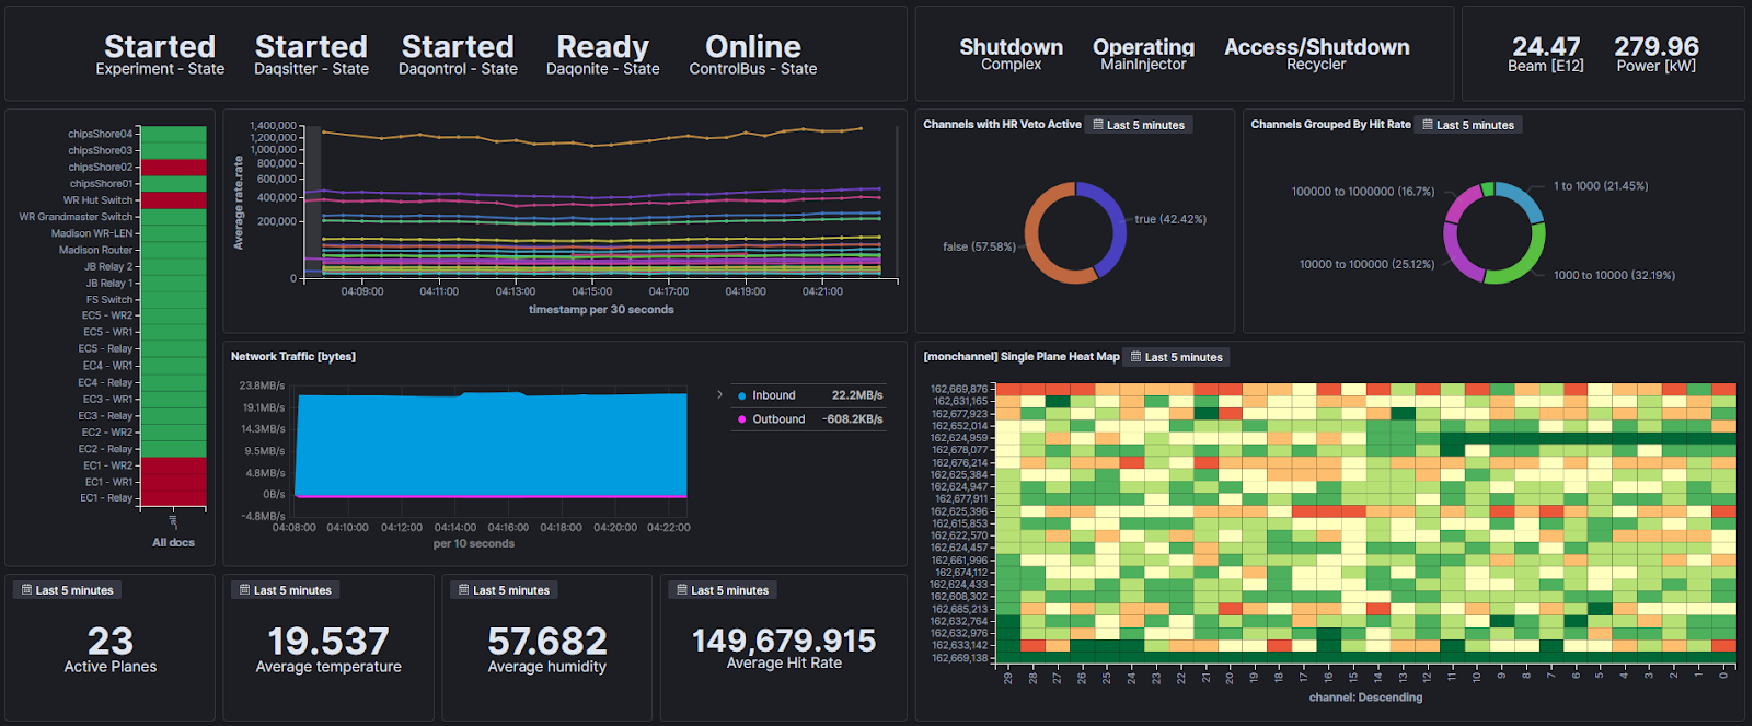
\includegraphics[width=\textwidth]{diagrams/5-daq/monitoring.pdf}
    \caption[Screenshot of a Kibana monitoring dashboard for \chipsfive]
    {Screenshot of a Kibana monitoring dashboard for \chipsfive. The dashboard pulls live
    monitoring data from the Elasticsearch database for its visualisations. The status of the
    various DAQ software components are shown in the top left above an average hit rate plot for
    each \textsc{Pom} and the colour coded status indicators for various DAQ devices. A plot of
    the network data rates is also shown alongside global average indicators. The right hand side
    of the dashboard contains visualisations to monitor the overall status and specific hit rates
    of PMTs.}
    \label{fig:monitoring}
\end{figure}

Furthermore, an alerting system using the ElastAlert framework~\cite{elastalert2020} provides
automatic notification of events for human attention. The ElastAlert process continuously checks
the Elasticsearch monitoring data for any breaches of predefined rules ($x$ events in $y$ time,
for example). Upon the occurrence of a rule trigger, multiple forms of notification (email and
Slack messages) are sent to appropriate recipients for further analysis and response.

Not only is the \chipsfive monitoring system extensible and easy to use it also has the advantage
of leveraging the efforts of an active open source community. With no additional effort by the
members of the \chips collaboration, the monitoring implementation will continue to improve with
time as updates are made to the underlying Elastic Stack software. This is likely to include both
performance improvements alongside new ways of quickly ingesting data and creating visualisations.
The monitoring approach firmly achieves one of the driving principles of the \chips project, using
commercially available, cheap (free in this case) components, wherever possible.